\chapter{Related Work}
\label{ch:related_work}


In this chapter, we review approaches made towards handling the Known-item Search (\acrshort{kis}) task and the recent approaches for user-friendly traverse through the immense amount of the visual data.

In the recent years, we have witnessed a significant advancement in frameworks focusing on the KIS task. An overview of the Video Browser Showdown evolution in the past few years is summarized in \citep{lokovc2018influential}. The scale of the frameworks' complexity for user interaction ranges from simple ones (e.g., sketching color blocks) with only a few descriptors to the ones which use recent advances in deep learning, for example, concept labeling.

Our goal is to perform a known-item-search task on a set of images. Developing a successful technique to approach the image KIS task can lead us to solve the KIS task over videos. We can perform the image search over the extracted frames from the videos. In our case, we used videos as a source for our dataset of images. More information on the dataset is presented in section \ref{s:dataset}.

At the end of this chapter, we provide an overview of the face recognition topic. We link to the recent overviews of the most successful systems based on deep neural networks.

\section{Known-item-search Task}

The known-item-search task is present in any multimedia format. We may look for a particular article in the database of the newspaper or for a specific photo in family album. This thesis focuses on visual KIS task; specifically, we retrieve images. In this chapter we review a few of the systems for the visual KIS task presented at the last \acrshort{vbs}2019. We mainly follow the summarization from \cite{rossetto2020interactive}. As the study presents, the most popular approach at the VBS2019 was \emph{Query by an Image} and \emph{Concept Labeling}. 

Query by an image in this case mostly refers to finding the most similar results from a database to a given image. The downside of this approach is the difficulty of obtaining an image that is sufficiently similar to the searched one.

Another widely used approach at VBS2019 was Concept Labelling. In this case, user describes the image by words. Firstly, the items in the database, are annotated by a variety of automatic tools. Then for each textual input query, the system checks the database for the presence of images with assigned labels matching the query. Concept labeling often faces a limitation on the vocabulary size, and accuracy issues caused by a classification misses. Recent advancements in the textual annotation by neural networks helped to tackle this problem. Nowadays, automatic annotation systems are able to classify thousands of different entities. However, even in so many classes we may not find a word to describe rarely used objects.

One of the other presented approaches is creating a color sketch. The user draws the sketches on the canvas which resembles the searched scene. The database is then searched for images with corresponding color patches. As a significant advantage of this approach, we see its ability to incorporate spatial information by searching for a specific color in a specific region of the image.
 
Solving the \acrshort{kis} task in the \acrshort{vbs} setting offers the option of using full video information and not only separate images. This approach allows for usage of additional techniques such as Temporal Queries or Multimodal queries. Also, some of the frameworks presented included Optical Character Recognition (OCR).

We designed our techniques as a possible enhancement for a complex system in order to support multiple search strategies based on a user-preference. At the same time, we present a standalone application to preview the described techniques.

\subsection{Traversal Approaches}

\acrshort{kis} task is the task of two sides -- the algorithm and the user. It is essential not to forget about the user experience. Smooth user experience with quick navigation over a dataset can help to find the target image faster. As the review of the \acrshort{vbs} by \cite{rossetto2020interactive} shows, the most common approach is to show a 2D grid of frames to the user. Several approaches also provide an easy way to play the original video. 

The traversal systems often rely on effective visualization techniques for high-dimensional data. Many of the frameworks presented at VBS create a 2D grid of images. The images in the grid are usually organized based on their high-dimensional representation, often produced by neural networks. 


\section{Overview of the existing frameworks}

In the next section, we shortly investigate some of the existing frameworks, which competed in the Video Browser Showdown. 

\subsection{VIRET}

A framework named VIRET [\cite{lokovc2019framework, lokovc2019viret}, see figure \ref{fig:viret}] has been successfully participating in the competitions for several years now. The framework has evolved throughout the years, and now it offers a wide variety of strategies for solving the KIS task. VIRET also implements its own strategy for a frame selection, which we also used for obtaining our images. As one of the most significant strategical advantages of the VIRET, we consider the option to use multimodal and temporal queries. Some of the features included in the tool are: search by color regions, video playback, key-word search, search by an example image. For the purposes of the Lifelog Search Challenge \citep{LSC20} the videos can be also searched by the meta-attributes (e.g., day of the week, time of the day). We take an inspiration from VIRET, although we do not implement the same approaches as there are already present in the VIRET. We focus on testing new alternatives.

We highly recommend more thorough description of the VIRET tool presented in \cite{kovalvcik2020viret}.

\begin{figure}
    \centering
    \includegraphics[width=\linewidth]{img/viret_overview.pdf}
    \caption{Example search in VIRET framework. Source: \cite{kovalvcik2020viret}}
    \label{fig:viret}
\end{figure}

\subsection{SOM-Hunter}

A SOM-Hunter was for the first time introduced at the \acrshort{vbs}2020. This tool is related to our approach because it also supports Self-organizing Maps to solve a Known-item-search task. The typical workflow (as described in \cite{kratochvil2020som}) starts with search based on the keywords. This reduces the dataset only to relevant images. During the entire browsing session, they preserve relevance score for each image. To display the results, they use a mapping onto a trained self-organizing map weighted by the relevance scores or a grid view sorted by the relevance scores. The user can continue to explore the dataset further by browsing or they also can reformulate the query. For more exploitation it is possible to browse over provided results. Since the showed displays are relatively small ($8\times8$ images when using a \acrshort{som}), the corresponding self-organizing map can be computed quickly. The user can also explore the temporal context of any of the images. A sample interaction with the system is displayed in \autoref{fig:som_hunter}.


\begin{figure}
    \centering
    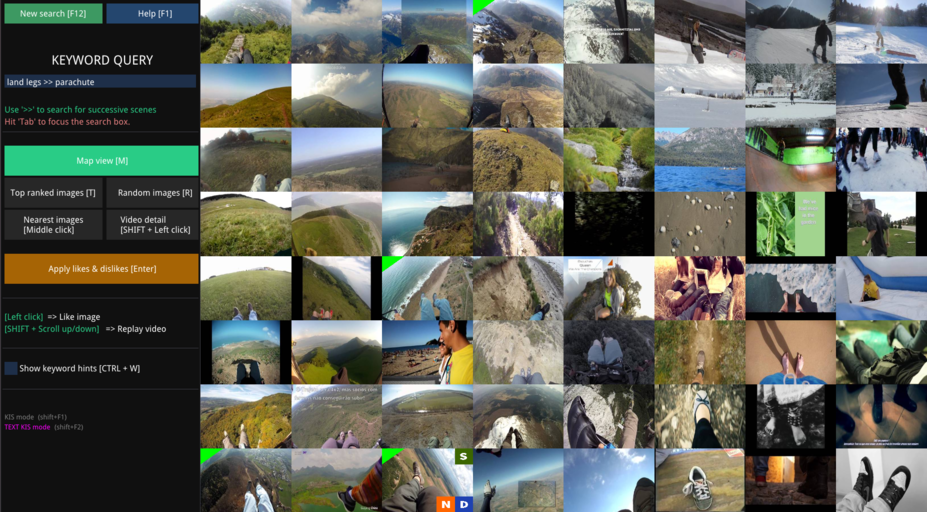
\includegraphics[width=0.99\linewidth]{img/som_hunter_small.png}
    \caption{A sample search in SOM-Hunter. Source: \href{https://videobrowsershowdown.org/hall-of-fame/}{Video Broser Showdown, Hall of Fame}}
    \label{fig:som_hunter}
\end{figure}

\subsection{Vitrivr}

Vitrivr [\cite{rossetto2016vitrivr}, \autoref{fig:vitrivr}] is a sophisticated framework for retrieving a video in the collection. Vitrivr is separated into three modules, Vitrivr-ng, Cineast, and Cottontail-DB.  Vitrivr-ng is the module responsible for creating queries that are later processed by the Cineast. Cottontail-DB supports fast retrieving methods of the features required by Cineast. The overview of the system is displayed in figure \ref{fig:vitrivr}. Vitrivr supports different query types: query by a sketch, as well as example image, semantic concept, keywords, audio, or motion. The feature extraction and the system behind retrieving the most similar results are parts of the second module -- Cineast (\cite{rossetto2016searching}). Cineast uses multiple approaches incorporating deep features, e.g., scene text recognition and speech-to-text recognition. Vitrivr-ng (the part responsible for creating the queries) is a web-based software. The modules structure provides a clean separation between the query formulation and feature extractions.

\begin{figure}
    \centering
    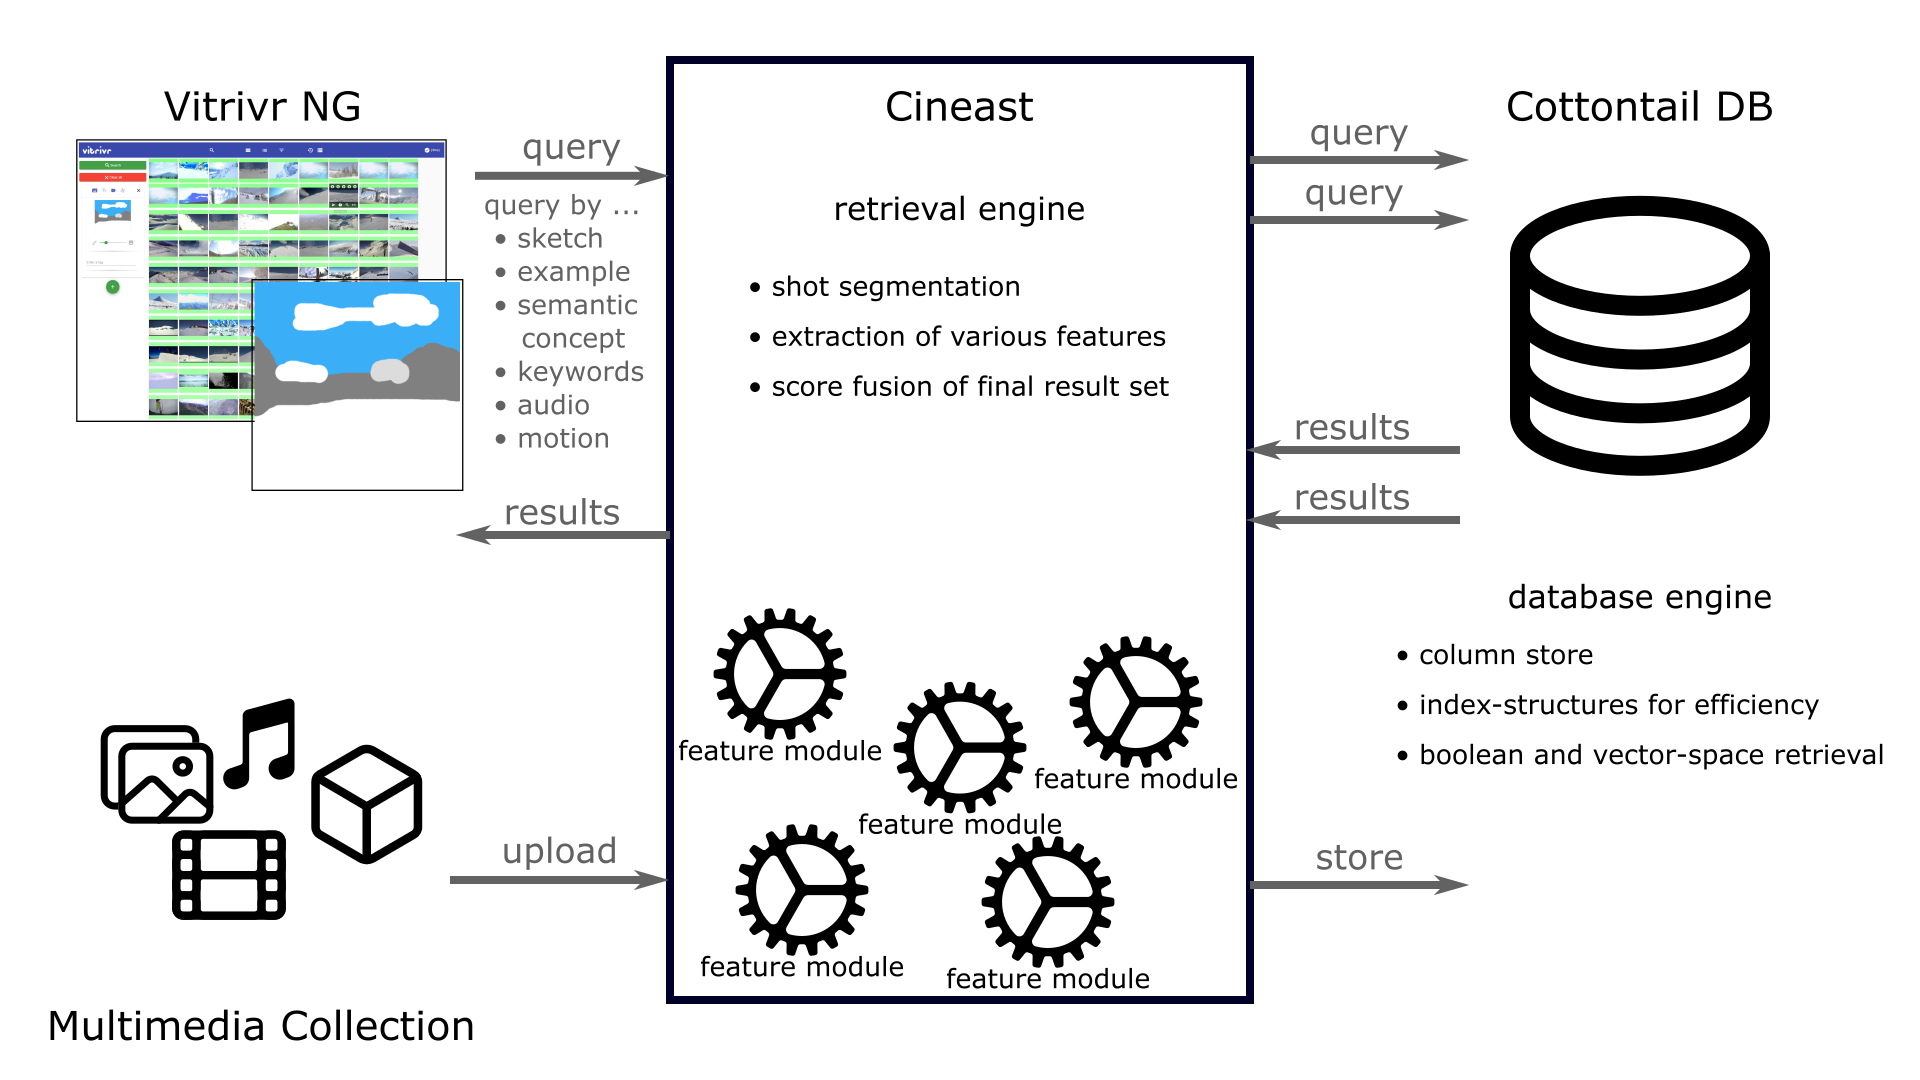
\includegraphics[width=\linewidth]{img/vitrivr.png}
    \caption{Overview of the separation in the Vitrivr framework. Source: \url{https://vitrivr.org/vitrivr.html}}
    \label{fig:vitrivr}
\end{figure}

\section{Face Recognition}

In the second part of the thesis, our goal is to organize faces to allow a faster search through the dataset. We leverage the face recognition technology to organize the faces into a hierarchical structure. One such approach is presented in \citep{girgensohn2004leveraging}. The authors' algorithm provides user with faces based on the similarity to existing models (i.e., person). They examined the performance of the model by a series of simulations. 

In the recent years, many steps have been taken towards solving the face recognition task. As the \cite{ranjan2018deep} overviews, three separable modules are typically needed for automatic verification and identification systems. Firstly, a face detector is applied to localize faces in images. A robust detector should be able to detect faces with a varying pose, illumination, and scale. Also, the bounding boxes of the detected faces should be minimized, to contain a minimal amount of background. Secondly, a landmark detector is usually incorporated. This detector localizes the important facial landmarks such as nose tip, mouth corners, etc. These points are then used to rotate and scale the face, which creates a normalized input for the next phase. Lastly, a feature descriptor encodes information from the aligned face. Based on these encodings and various similarity measures, the model can signify if the two faces belong to the same person or perform other related tasks.

The face recognition problem can be further split into two categories: face verification and face identification. In the face verification task, the goal is to determine whether two subjected faces belong to the same person. In the identification scenario,
a set of known subjects is inserted into the system. Then, a new subject (target) is presented. The goal of the model is to retrieve all faces from the dataset belonging to this person, or in supervised manner, to assign the identity.

Since the early 1990s, many face identification/verification systems were proposed. For example, in \citep{kalocsai1998face}, authors conducted a study, where two faces were shown to the respondents, simulating the verification task. Then, the respondents were asked to decide if the faces belong to the same person. The faces displayed a different emotions. The researchers suggest that the model's performance correlates with the subjective human representation of the faces.

Twenty-five years later, with the advancements of the deep neural networks, new state-of-art methods achieve an almost perfect score on some of the benchmarks (e.g., \citep{huang2008labeled}). We refer to the \citep{masi2018deep} to provide an overview of the recent models used for face identification and verification. The summary also provides a thorough description of the individual steps usually taken by the approaches presented. In our work, we use pre-trained models provided by the dlib library. We include more technical information in section \ref{s:dlib}.

\section{Dataset}
\label{s:dataset}

We use Vimeo Creative Commons Collections (V3C1)\footnote{\href{https://www-nlpir.nist.gov/projects/tv2019/data.html}{TRECVID 2019 Video Data}} dataset for experimenting and evaluations. This dataset is used for evaluations at \acrshort{vbs} and also at TRECVID. The dataset is composed of 7475 Vimeo videos. We selected only the first 750 videos for proving concepts of our work. From these 750 videos, 111\ 764 images were extracted with resolution 320x180 by using an extraction tool from \cite{lokovc2019framework}. I extend my gratitude to Tomáš Souček and Gregor Kovačík for providing extracted images.

The videos capture a wide range of sceneries on many different occasions. We can see many different landscapes, from seas to mountain views, from desert to snow. A large proportion of the videos contain people. Videos capture people doing different activities, e.g., Hindi wedding, skateboarding in a park or a news broadcast.


\chapter{Theoretical and Technical Background}
\label{ch:technical_background}

This chapter intends to review the fundamentals of the theoretical approaches used in this thesis. It includes the fundamental concepts of neural networks and a short description of the networks we use. The chapter also reviews projection methods of high-dimensional data to lower-dimensional space.

\section{Deep Neural Networks}

In recent years we witnessed emergence of many records-breaking machine learning models. Many of those breakthroughs were possible thanks to the advancement of Deep Neural Networks (\acrshort{dnn}). Nowadays, these models replaced more traditional Machine Learning approaches in many tasks.

Deep Neural Network is a machine learning model, whose goal is to approximate a given function \(f\). The set of its parameters is often referred to as \(\theta\). One of the everyday tasks performed by these networks is classification, where the goal of the network is to predict which category sample \(X\) belongs to. Even though we will not perform a classification task in this thesis, we will use some of the available classification networks.

When we talk about neural networks, we usually refer to a feedforward network. These networks consist of layers which only pass information in one direction during the evaluation. We can imagine it as applying a function to the results from the previous layer. For example, let us create a small neural network. Denote first layer as \(f_1\) and second layer as \(f_2\). The output of the network will be \(f_2\left(f_1\left(\cdot\right)\right)\).

Stacking more and more layers on top of each other leads us to the notation \emph{deep} neural networks. This notation has no fixed threshold on which networks ``deserve'' to be called deep. The word ``deep'' separates the eras between the neural networks consisting of a couple of layers from neural networks consisting of tens or more layers.  

The first and last layer are commonly referenced as an \emph{input} and \emph{output} layer, respectively. Layers between the input and output layers are usually denoted as \emph{hidden} layers. Deep neural networks can have four or hundreds of layers, and there are multiple types of operations that layer can perform. \emph{Network Architecture} captures the ``build order'' of the network. It is important to note that there exist many networks with different architectures solving the same task.

There are many reasons for the advancement of neural networks in the past years. One of the crucial stones was not only theoretical innovations used for the networks but increasing computability limits. Deep Neural Networks \emph{learn} to approximate function by \emph{training}. This training is usually the heaviest part of the computation. Even though it is enough to train it once and use forever, it usually lays some limitations on the size of the networks or the functions used.

Since this topic is broad, we recommend more thorough reading, such as Neural Networks and Deep learning online book \citep{nielsen2015neural}.

\subsection{Convolution Neural Networks}

Convolution Neural Networks (\acrshort{cnn}) are a class of Deep Neural Networks. Even though they emerged in the late 1980s \citep{lecun1989backpropagation}, it took another 20 years for further advancements in the research area. Convolution Neural Networks are mainly used in image-related tasks, such as image classification (``What is on the image?''), object detection (``Where are the objects in the image and what are they?'') or even content generation (``Create a new image''). Their abilities were also tested in many, not image-related tasks, e.g., music genre recognition.

Convolutional Neural Networks are specialized kind of networks which usually work with grid-like topology. For 2D case, most typically image pixels represent a grid. The name \emph{convolution} refers to using a mathematical linear function \emph{convolution} in at least one of the layers. A simplified overview of the structure is displayed in figure \ref{fig:convolution_neural_network}. We refer to \cite{Goodfellow-et-al-2016} for additional information about the \emph{convolutional layers}.

\begin{figure}
    \centering
    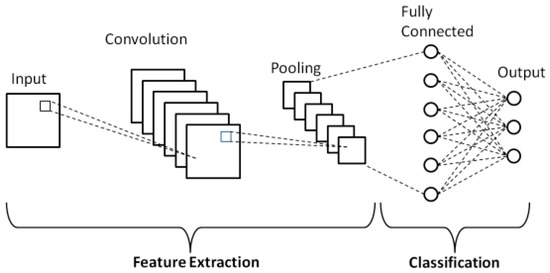
\includegraphics[width=0.98\textwidth]{img/convolution_neural_network.jpg}
    \caption{Schematic diagram of a convolutional neural network. Source: Phung, V.H.; Rhee, E.J. A High-Accuracy Model Average Ensemble of Convolutional Neural Networks for Classification of Cloud Image Patches on Small Datasets. Appl. Sci. 2019, 9, 4500.}
    \label{fig:convolution_neural_network}
\end{figure}

% \todo[inline]{pooling}
% \todo[inline]{convolution block}

\subsection{Transfer Learning}

Transfer Learning is a research problem in machine learning that focuses on storing knowledge gained while solving one problem and applying it to a different problem. We have seen many successful transfers of the network architecture and parameters learned to a new task. Transfer learning may help to reduce the cost of the training and often also to overcome an insufficient set of training examples for the new task.

We utilize some of the pre-trained Convolution Neural Networks. The possibility of using a pre-trained neural network on a different task than they were trained on was explored as early as 2014 by \cite{donahuedeep}, and many others were able to use this process to acquire better models.  Networks we use are mostly pre-trained on \emph{ImageNet}\footnote{http://www.image-net.org/}. ImageNet serves as one of benchmarks for comparing the performance of the different networks. Since the ImageNet Challenge is a classification task, we utilize the transfer learning to obtain deep features, by stripping the last classification layer. Layers at the end of the networks accumulate semantic information, i.e., they contain high-level features. Therefore, we work with the layers close to the output layer. These layers represent encoded information about the image in high dimensional vectors. Our task is to use these deep features obtained for solving our known-item search task.

\begin{figure}
    \centering
	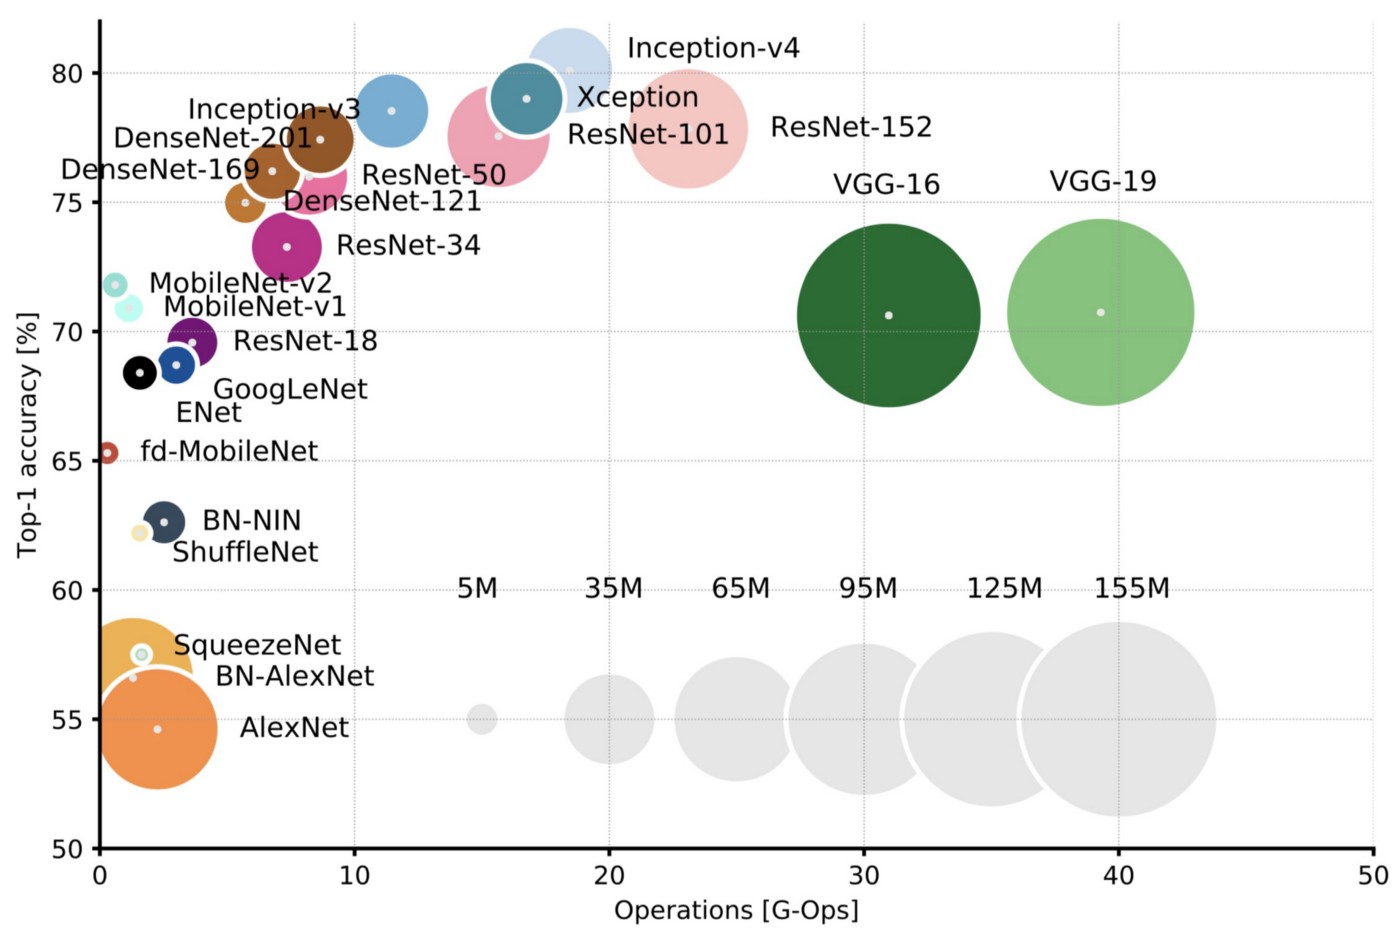
\includegraphics[width=0.8\linewidth]{img/network-comparison.jpeg}
	\caption{Top-1 one-crop accuracy versus amount of operations required for a single forward pass. The size of the blobs is proportional to the number of network parameters. Source: \cite{canziani2016analysis}}
	\label{fig:camera-setup}
\end{figure}

\subsection{Pretrained models}
\label{ss:pretrained_models}

In our work we use various pretrained models. We obtain the models from Keras, Dlib, or other open sourced projects. In the following sections we describe the frameworks and libraries we use.

\subsection{Keras}

Keras \citep{chollet2015keras} is a deep learning \acrshort{api} written in Python, running on top of the machine learning platform TensorFlow \citep{tensorflow2015-whitepaper}. It was developed with a focus on experimentation in deep learning. We use it and its pre-trained models in this thesis. The models, which we use from Keras Applications, were trained on ImageNet. Keras API allows us to remove the last fully connected layer used for classification (since default ImageNet is a classification task) from the selected neural network.

In this thesis, we use pre-trained models to implement new approaches. We do not aim to train new models or further train existing ones. We try to extract the information from available models to solve the known-item search task. Here we describe two models which we experimented with the most. ResNet was a state of the art model as of 2015. Since then, it gained popularity in many tasks. The second network we focus on is MobileNet. MobileNet has an excellent performance to complexity ratio. Therefore, it is an ideal network for our purpose where the predictions need to be computed online and displayed to the user.

\subsection*{Resnet50V2}

ResNet (abbv. for Residual Networks, \cite{resnet}) is a classic neural network used in many computer vision tasks. ResNet was the winner of the ILSVRC 2015 (\citep{ILSVRC15}). The authors aimed to solve a problem of degrading training accuracy of the neural networks, when more layers were added. 

The authors argued that the reason behind the degradation is that approximating identity function by a layer in a neural network is difficult (otherwise the added layers should learn to approximate identity and resulting error should be no greater then when using shallower counterpart). To solve this problem they, instead of trying to approximate underlaying mapping $H(x)$, they ask the neural network to approximate residual function $F(x)=H(x) - x$. That way if identify is suitable function the weights just needed to be driven to zero (achieve $0 = H(x) - x$ i.e. $H(x) = x$). They do so by replacing simple layers by residual building blocks (see figure \ref{fig:resnetv2}).

\begin{figure}
    \centering
    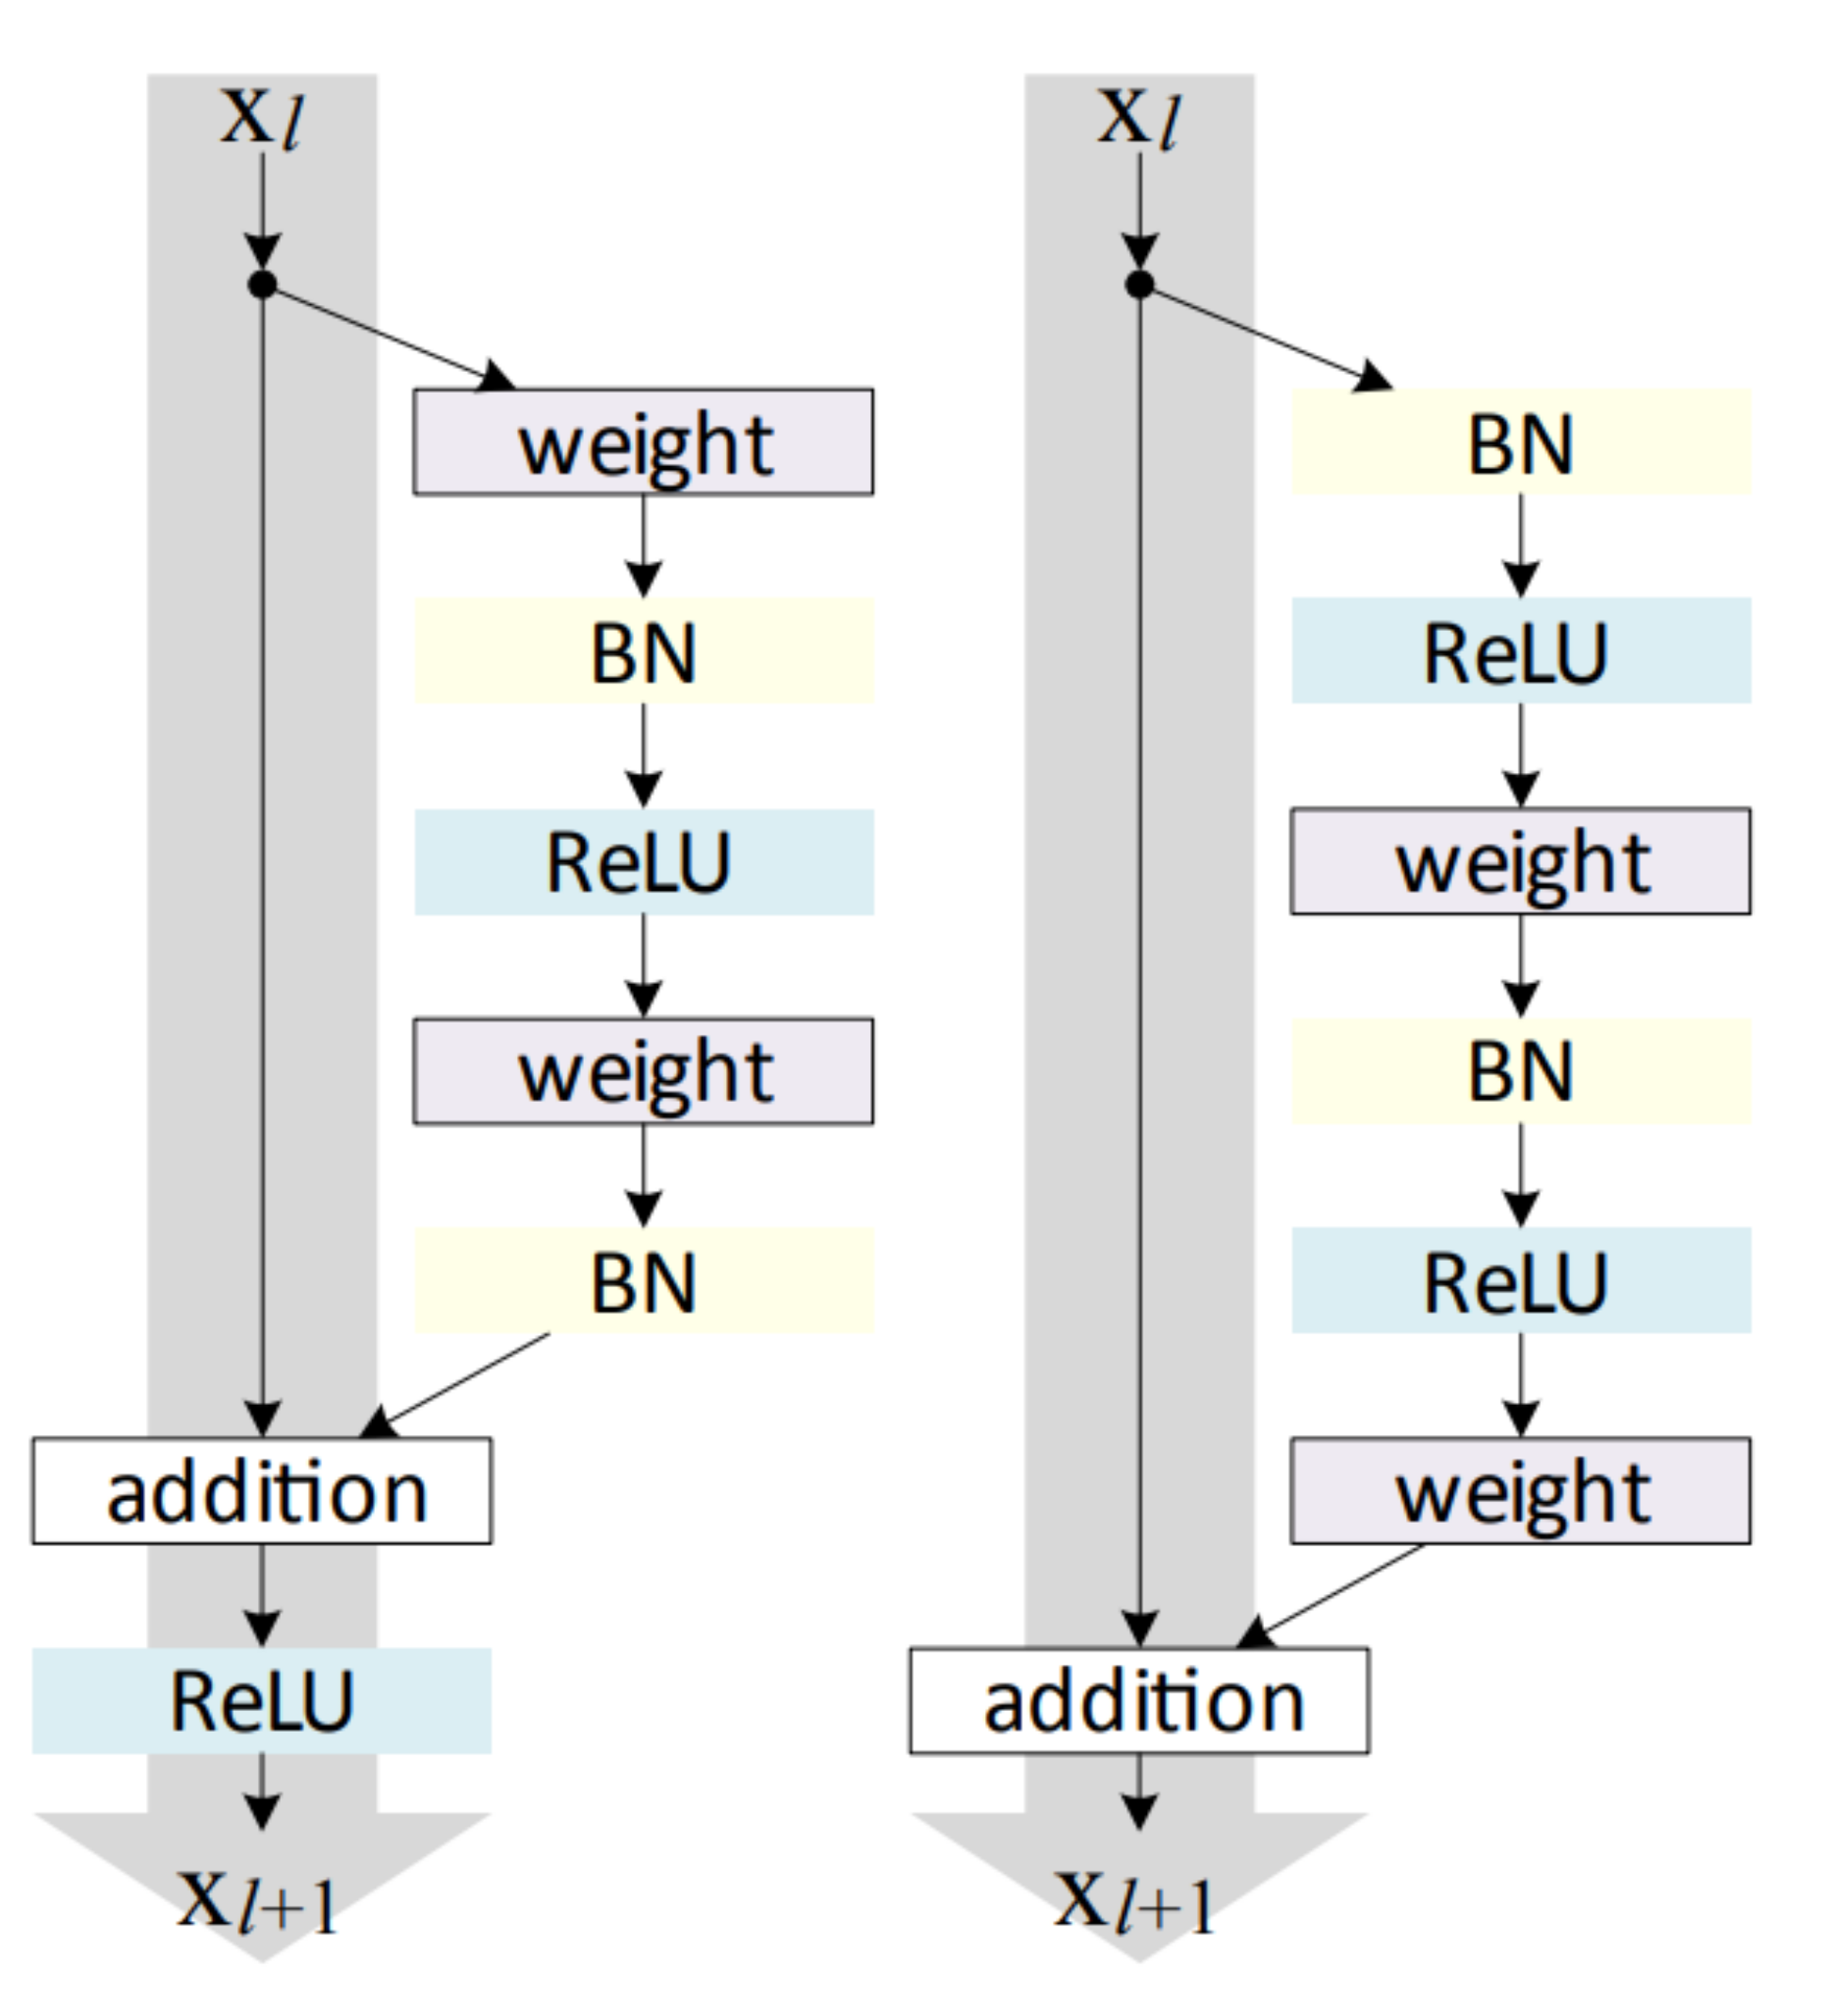
\includegraphics[width=0.5\textwidth]{img/resnetv2.png}
    \caption{Left: ResNet residual unit as proposed in \citep{resnet}. Right: ResNetV2 residual unit by \citep{resnetv2}. Source: \cite{resnetv2}}
    \label{fig:resnetv2}
\end{figure}

In \citep{resnetv2}  the authors improved the architecture of ResNet by changing the position of activation an batch normalization layers. By doing so they made the easiest path for the information to propagate even simpler. For details see the figure \ref{fig:resnetv2}. This improved architecture is commonly known as ResNetV2.


% ResNet (short for Residual Networks, \cite{resnet}) is a classic neural network used in many computer vision tasks. ResNet was the winner of the ImageNet challenge in 2015. ResNet architecture allowed training deeper networks, which was not possible before because of vanishing gradients. ResNet's main idea is to allow ``skipping connections'' between the layers. This has two main reasons: it mitigates the problem of the vanishing gradients and allows learning an identity function for higher layers in the network. ResNetV2 \citep{resnetv2} was released as an improvement of the ResNet. It included batch normalization and ReLU activation prior 2D convolution layer. 

% ResNet is still well-known and popular among the machine-learning community. Several pre-trained models are available, and it has well-tested implementations. We use it in the thesis for some experiments, although we prefer MobileNet due to shorter prediction time.

\subsubsection*{MobileNetV2}

In April 2017, a group of researchers from Google published a study \citep{mobilenet} introducing a new neural network architecture. This MobileNet was optimized for mobile devices. They optimized the model to deliver high accuracy while keeping the model and mathematical operations as fast as possible. Not a year later, MobileNetV2 was introduced by \cite{mobilenetv2}. It extended the predecessor by using Inverted Residuals with Linear Bottlenecks. For more details, please refer to the original research. In our work, we use only MobileNetV2 out of MobileNets.


\subsection{Dlib}
\label{s:dlib}

Dlib \citep{king2009dlib} is a modern C++ toolkit containing machine learning algorithms and tools for creating complex software in C++ to solve real-world problems. We use the Dlib library for face detection and also face feature extraction. For both, we use Python \acrshort{api} provided by \verb+face_recognition+ \citep{geitgey2016machine}. 

\subsubsection*{Face detection}

The authors of dlib implemented two key approaches to face detection. The first one, the frontal face detector, is based on the histogram of gradients. This approach is very fast in learning to detect the faces and also fast on performing the detections. It is still used in a variety of online tasks. The original release notes are available in \citep{king2017dlib_hog}.

The second approach present in the dlib is based on the convolutional neural network. This approach has longer inference time. However, based on evaluations, it has higher accuracy in non-frontal face views. The overview of both approaches is provided, for example, by \citep{arun2018cnndlib}.

\subsubsection*{Face encodings}

Dlib also presents a model for face encoding extraction. This model was trained for the face verification task. Based on published results (\href{http://vis-www.cs.umass.edu/lfw/results.html}{Labeled Faces in the Wild Benchmark}), the model achieves  99.38\% accuracy on the verification task. The network architecture is based on the ResNet34 and trained on the mix of the available datasets of faces. The review of the model is available at \citep{king2017high}.

\section{Principal Component Analysis}
\label{s:pca}

In projection methods for dimensionality reduction, the goal is to find a mapping of the input vectors from the original $d$-dimensional space to a new $k$-dimensional space (where $k < d$) with minimum information loss. \acrshort{pca} is one of such methods. It is an unsupervised method, which employs linear projection to decrease number of dimensions while preserving the explanation for variance within the data. Since the derivation of the formulas for \acrshort{pca} requires several technicals steps and some advanced knowledge of Linear Algebra, we refer to the \cite{alpaydin2020introduction} for a more detailed description.

\section{Self-organizing maps}
\label{s:som}

The self-organizing map was introduced by \cite{kohonen1982self}. The self-organizing map, abbreviated as \acrshort{som}, is an example of popular neural network based on unsupervised learning.  It produces low-dimension (typically two-dimension), discretized representation of the input space. Additionally, the \acrlong{som} structure forms a semantic map, where similar samples are mapped close together and dissimilar ones further apart.

The SOM consists of neurons $M$ organized on a regular low-dimensional grid. Each neuron is represented by a $d$-dimensional weight vector, where $d$ is equal to the dimension of the input vectors, we shall denote this mapping $\phi: M \rightarrow \mathbb{R}^d$. Each neuron is connected to the adjacent neurons by a neighborhood relation, which is induced by distance between their representations in the low-dimensional space and a threshold. This relation creates the structure of the map. 

During the training, the weight vectors are initialized with random values. Then, iteratively, we find the closest weight vector to a data point, called the Best Matching Unit (we denote such mapping $\mu: \mathbb{R}^d \rightarrow M$). We shift the weight vector of the \acrshort{bmu}, and usually also weight vectors of the neighboring neurons, closer to the data point. The impact on the neighboring neurons is usually scaled by the distance from the BMU.

The SOM can be thought of as net spread across the data. After the training, the neighboring neurons on the grid get similar weight vectors. For a more detailed description, please refer to \cite{kohonen1982self} and \cite{kohonen2007kohonen}. Extensive research on the topic of image retrieval using SOM was also presented by \cite{koskela2003interactive}.

Various measures have been developed to quantify a map's quality. In this thesis we use following two: quantization error and topographic error. For motivation behind the errors and more information about them, we refer to \cite{breard2017evaluating} and the original research. Here we present their definition and brief description.

\subsubsection*{Quantization Error}

A quantization error is formulated for example in \cite{wandeto2019quantization}. It is a measure of the average distance between the data points $x_i \in X$ and the map nodes to which they are mapped. The quantization error $QE$ for a map $M$ is calculated as follows:

$$
 QE(M) = \frac{1}{n}\sum_{i=0}^{n-1} ||\phi(\mu(x_i)) - x_i ||
$$

where $n$ is the number of samples in the training data $D$.
%$\phi$ is the mapping from the input space $D$ to the SOM $M$, i.e., it returns the weight vector of the BMU.

\subsubsection*{Topographic Error}

Topographic error was introduced by \cite{kiviluoto1996topology}. It accounts for a SOM's ability to preserve local topological features in a low dimensional output space. A sample for which the best matching unit and the second best matching unit are not adjacent counts as an error. The topographic error is given by the the total number of errors divided by the total of samples.

$$
    TE(M) = \frac{1}{n}\sum_{i=0}^{n-1}t(x_i)
$$

$$
    t(x) = \begin{cases}
			0, & \text{if $\mu(x)$ and $\mu'(x)$ are neighbors}\\
            1, & \text{otherwise}
		 \end{cases}
$$

where $\mu'(x)$ returns the second-best-matching unit.